\section{Numerical Experiments}

\begin{frame}{Burgers' \& Fisher-KPP Equations - Training Data}
    
  \begin{columns}[T,onlytextwidth]
    %===== Left column: Burgers figures =====%
    \column{0.48\textwidth}
    {\tiny $q_t + q\;q_x = \nu\;q_{xx},~~x\in[0,1], t\in[0,1],\nu=0.01$,\\
    $q(x,0) = \sin(2\pi x)$, BCs: Dirichlet }
    \begin{figure}
      \centering
      \begin{subfigure}[t]{\textwidth}
        \centering
        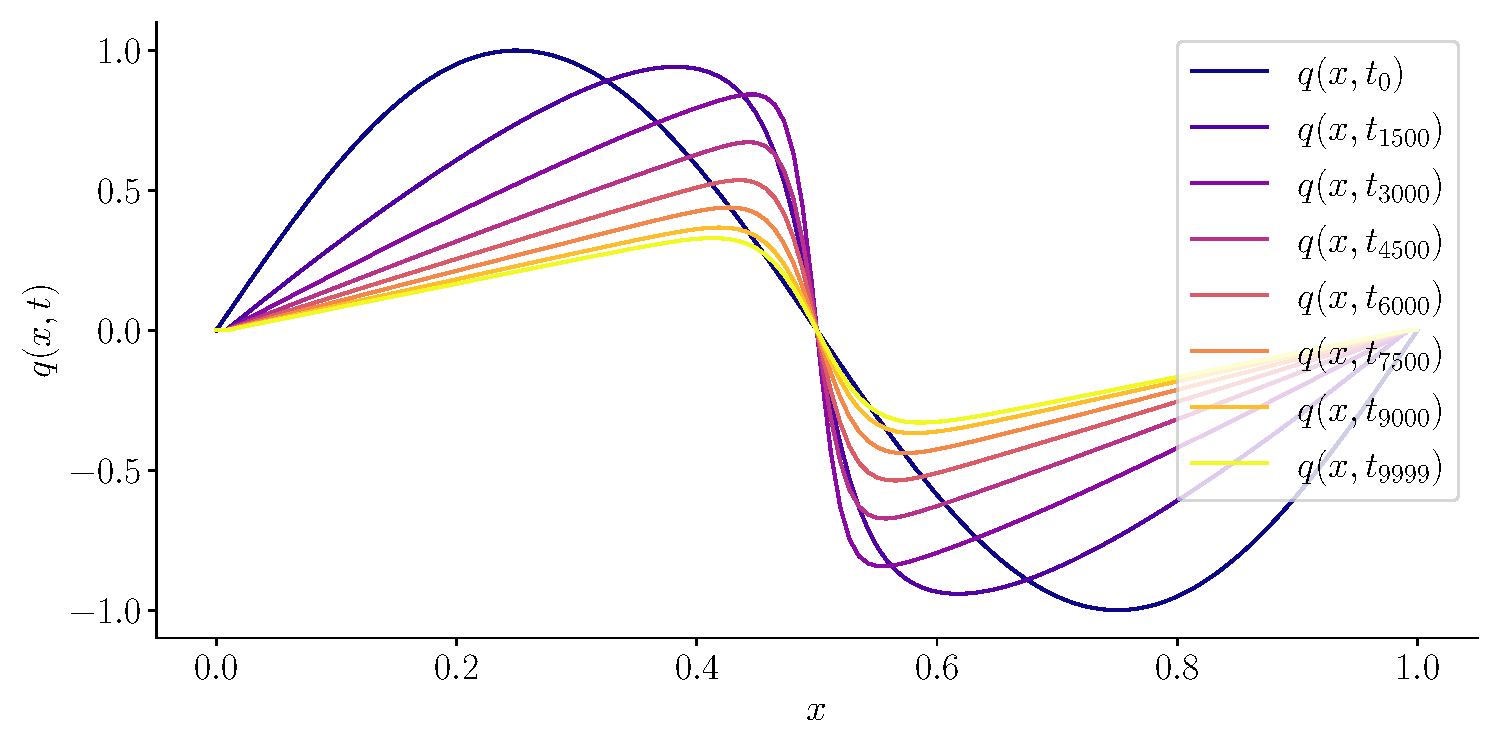
\includegraphics[width=0.7\textwidth]{images/burgers_evol_001.pdf}
        \caption{Profiles \(q(x,t_k)\) at selected times \(t_k\).}
        \label{fig:burgers-surface}
      \end{subfigure}
      \\[1em]
      \begin{subfigure}[t]{0.47\textwidth}
        \centering
        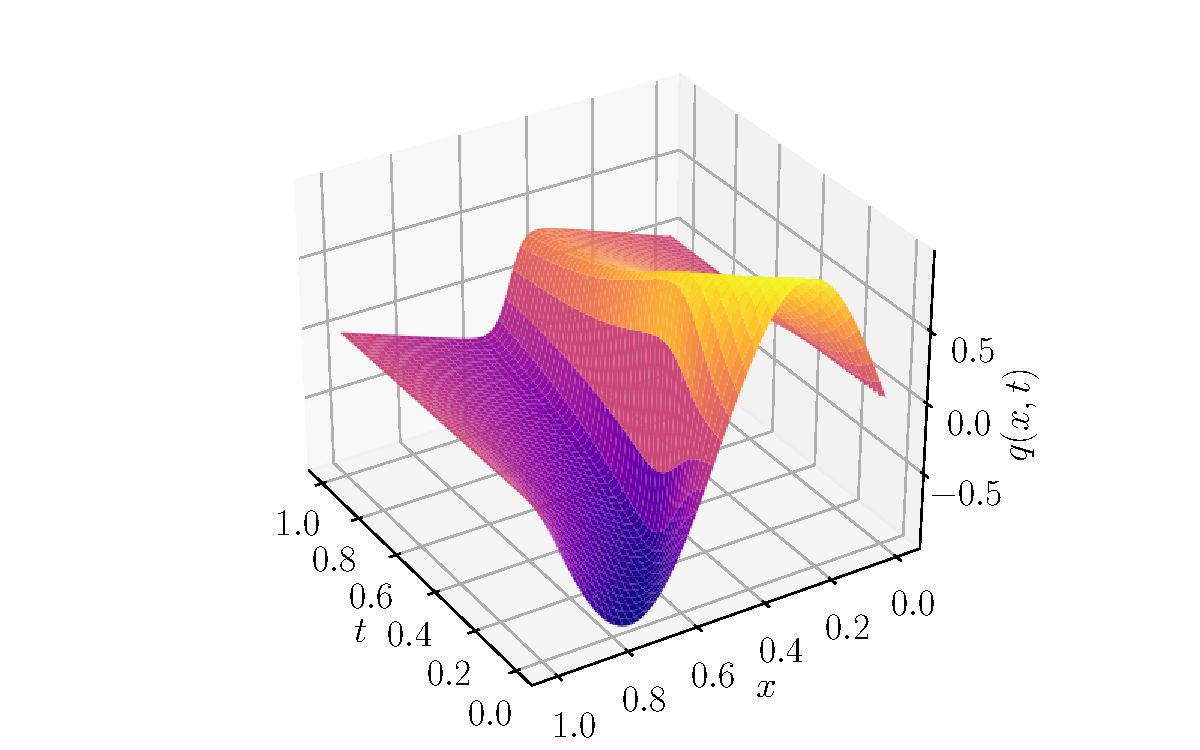
\includegraphics[width=\textwidth]{images/burgers_sol_001.pdf}
        \caption{\(q(x,t)\) for \(\nu=0.01\).}
        \label{fig:burgers-slices}
      \end{subfigure}
      \hspace{0.02\textwidth}
      \begin{subfigure}[t]{0.47\textwidth}
        \centering
        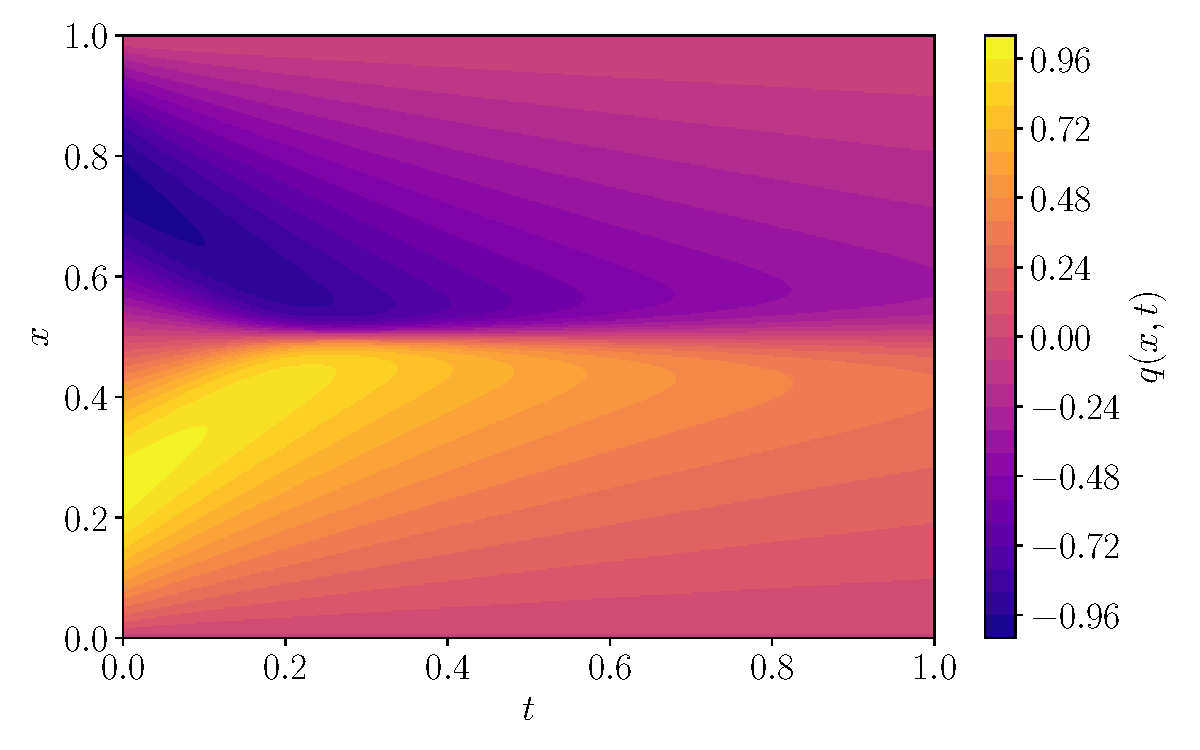
\includegraphics[width=\textwidth]{images/heatmap_001.pdf}
        \caption{Contour of \(q(x,t)\).}
        \label{fig:burgers-contour}
      \end{subfigure}
      \caption*{After FD discr. scheme $N_x=2^7,~\Delta t\approx0.0001 ~\!\!\Rightarrow\!\!~ \mathbf{Q}\in\mathbb{R}^{130\times 10000}$.}
      \label{fig:burgers-data}
    \end{figure}
    %%%%
    \column{0.02\textwidth}
    \centering
    \vrule width 0.36pt height 0.84\textheight
    %===== Right column: FKPP figures =====%
    \column{0.48\textwidth}
    {\tiny $q_t = \mathfrak{D}(q_{xx} +  q_{yy}) +\rho\;q(1-q),~~x,y\in[0,10],~t\in[0,5], ~\mathfrak{D}=0.1$,\\
    $\rho=1, ~q(x,y,0)=\exp(-10[(x-5)^2 + (y-5)^2])$, BCs: Neumann}
    \begin{figure}
      \centering
      \begin{subfigure}[t]{\textwidth}
        \centering
        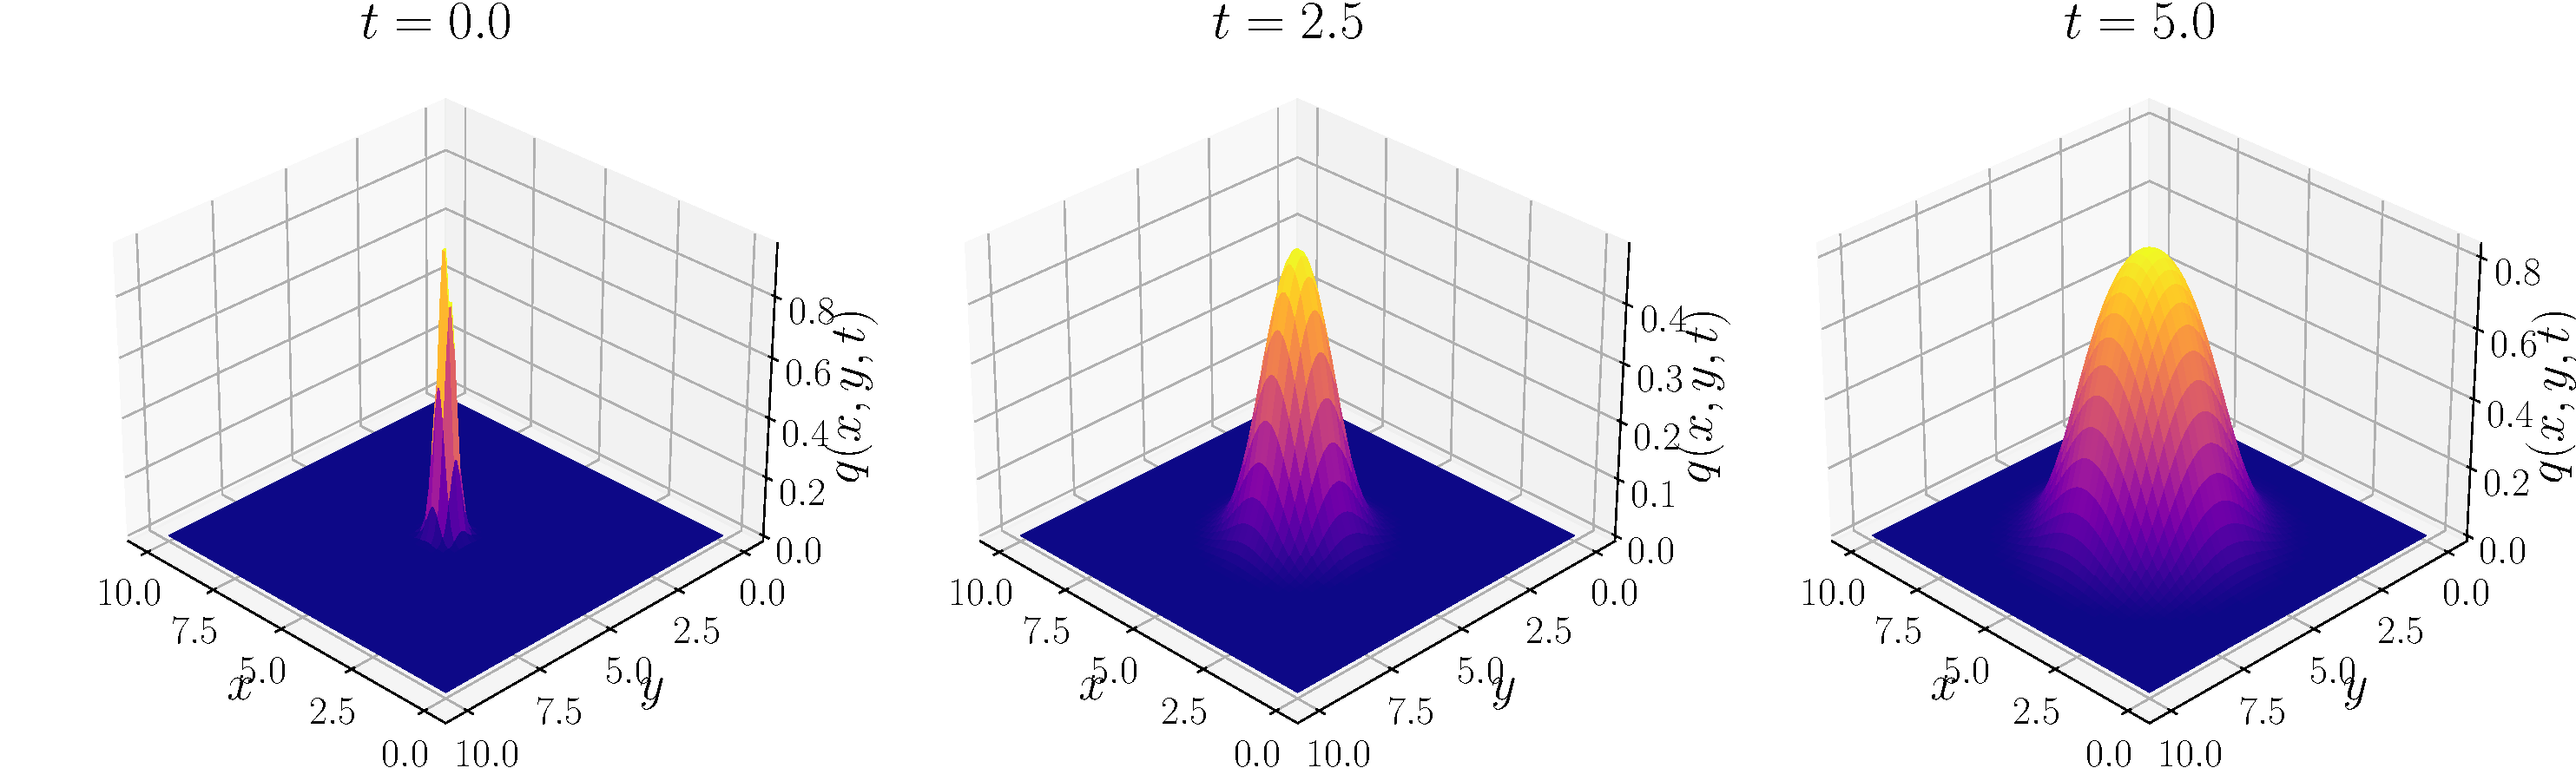
\includegraphics[width=\textwidth]{images/3Dfkpp.pdf}
        \caption{\(q(x,y,t)\) for \(\mathfrak{D}=0.1,\rho=1\).}
        \label{fig:fisher-init}
      \end{subfigure}
      \\[1em]
      \begin{subfigure}[t]{0.48\textwidth}
        \centering
        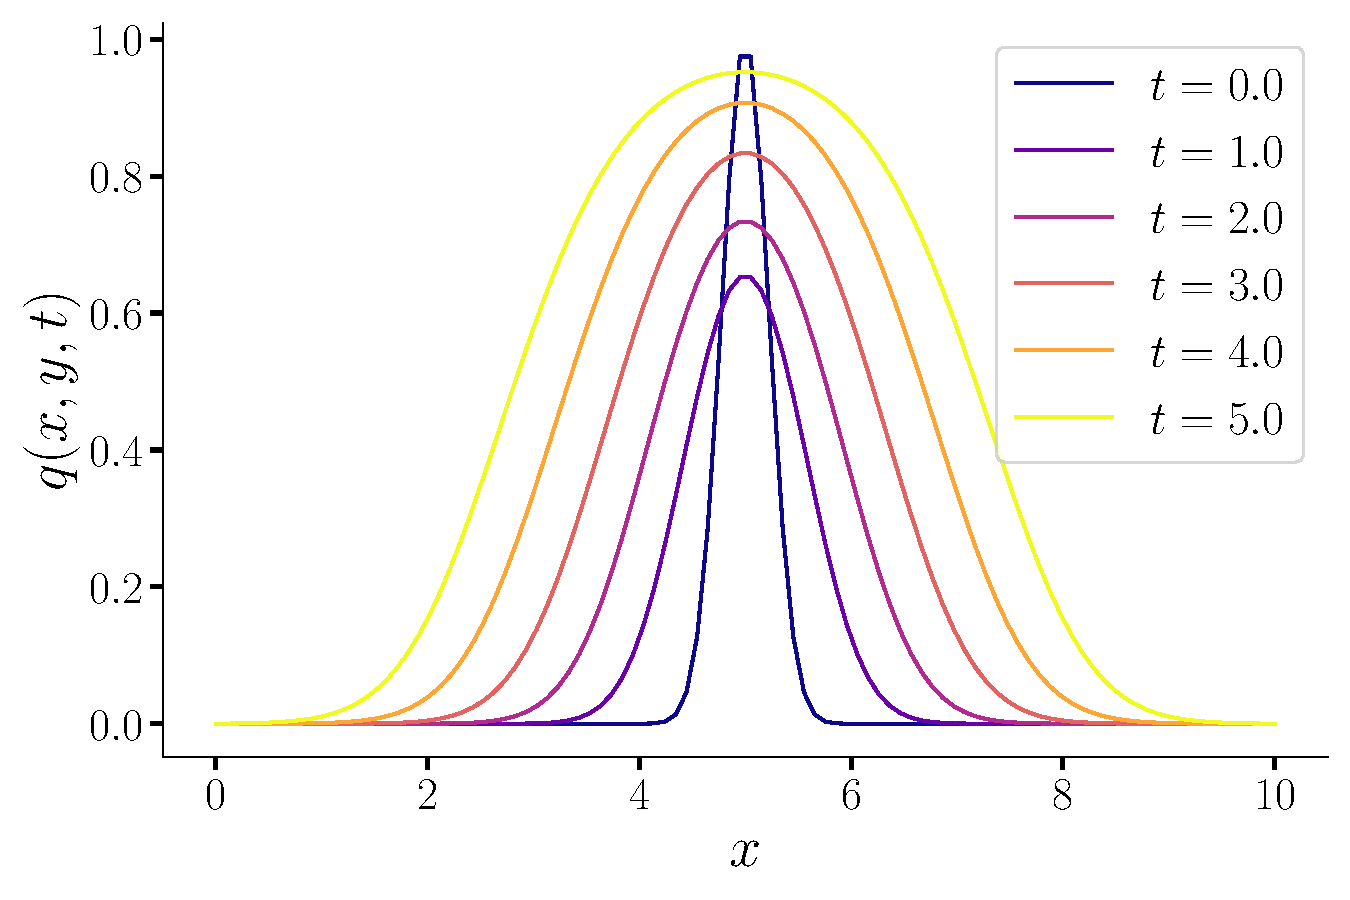
\includegraphics[width=\textwidth]{images/1Dfkpp.pdf}
        \caption{Profiles of \(q(x,y,t_k)\).}
        \label{fig:fisher-mid}
      \end{subfigure}
      \hfill
      \begin{subfigure}[t]{0.48\textwidth}
        \centering
        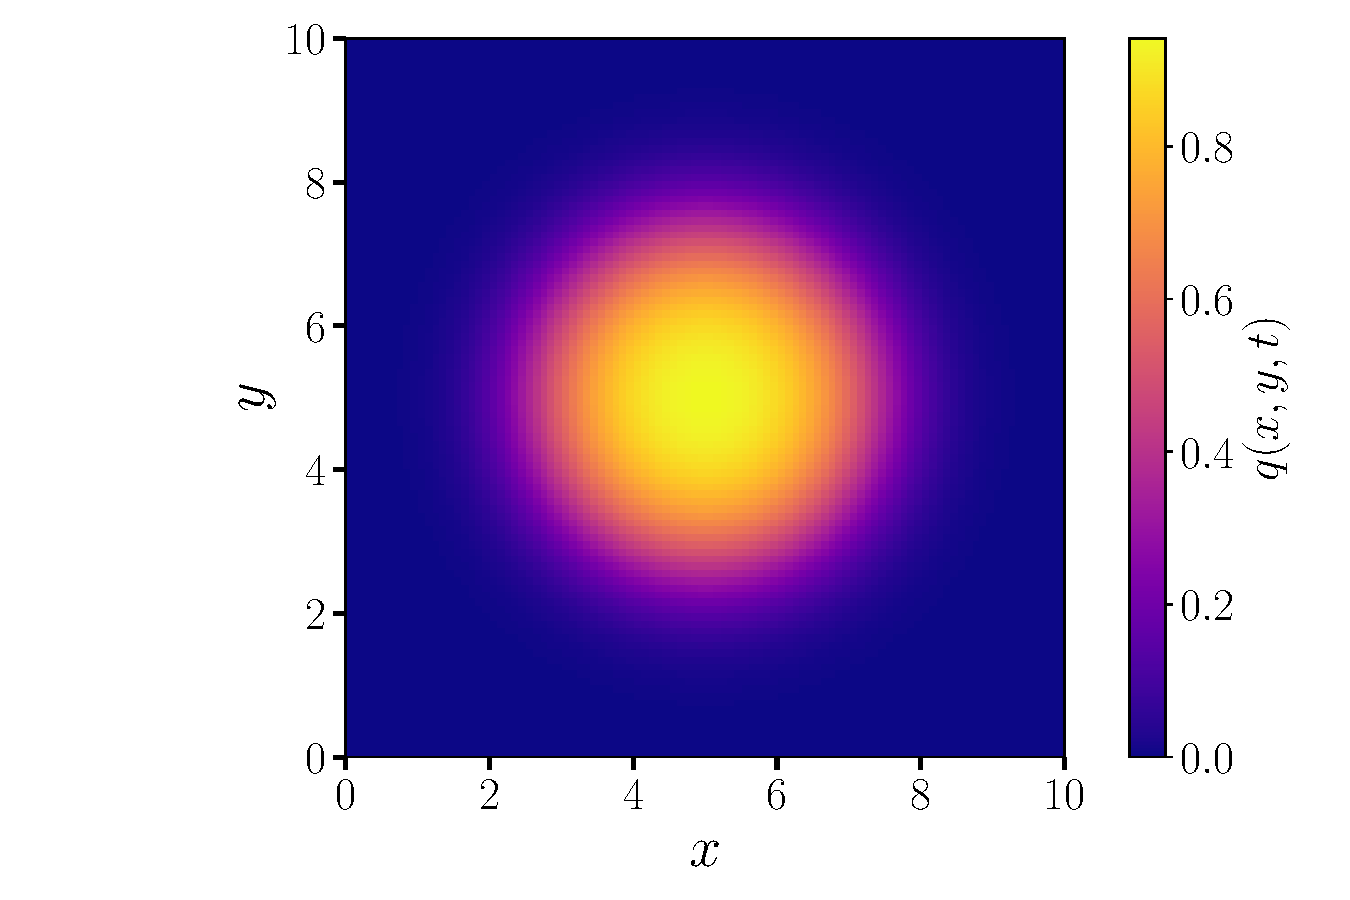
\includegraphics[width=\textwidth]{images/2Dfkpp.pdf}
        \caption{Contour of \(q(x,y,t=5)\).}
        \label{fig:fisher-final}
      \end{subfigure}
      \caption*{FD discr. with $N_x=N_y=100,~\Delta t = 0.005 ~\!\!\Rightarrow\!\!~ \mathbf{Q}\in\mathbb{R}^{10000\times 1000}$.}
      \label{fig:fisher-data}
    \end{figure}
  \end{columns}
\end{frame}


\begin{frame}{Burgers' Results I}

Data perturbation: $\displaystyle\text{noise}\sim\mathcal{N}(0, \sigma^2),\quad \sigma=\dfrac{\text{pct}}{100}\max_{1 \leq j \leq k} \left\| \mathbf{q}(t_j) \right\|_2
$

\vspace{0.6cm}

  \begin{columns}[T,onlytextwidth]  % top‐aligned columns, full text width
    \column{0.48\textwidth}
      \centering
      %
\includegraphics[width=\textwidth]{images/placeholder_image.png}
      \animategraphics[loop,autoplay,width=\textwidth]{1}{images/rom_noise_10-}{1}{2}
      %\captionof*{figure}{Left plot}
      \label{fig:left}

    \column{0.04\textwidth}
      % just a gutter; you can adjust or even draw a rule here

    \column{0.48\textwidth}
      \centering
      \animategraphics[loop,autoplay,width=\textwidth]{1}{images/rom_noise_20-}{1}{2}
      %\captionof*{figure}{Right plot}
      \label{fig:right}
  \end{columns}

\vspace{-0.3cm}

  \begin{table}[]
        \begin{tabular}{c|cccc}
            \textbf{Rel. State $\mathbf{L^2}$ Error} & 1\% & 5\% & 10\% & 20\% \\
            \hline\hline
            OpInf     &  0.04039634  & 0.04910057   & 0.05458478  & 0.16265746  \\
            Adjoint   &  0.03814659  & 0.03817415   & 0.03962203  & 0.08028812 
        \end{tabular}
  \end{table}
    
\end{frame}

\begin{frame}{Burgers' Results II}
    
\begin{figure}[h!]
  \centering
  
  % First row of subfigures
  \begin{subfigure}[b]{0.3\textwidth}
    \centering
    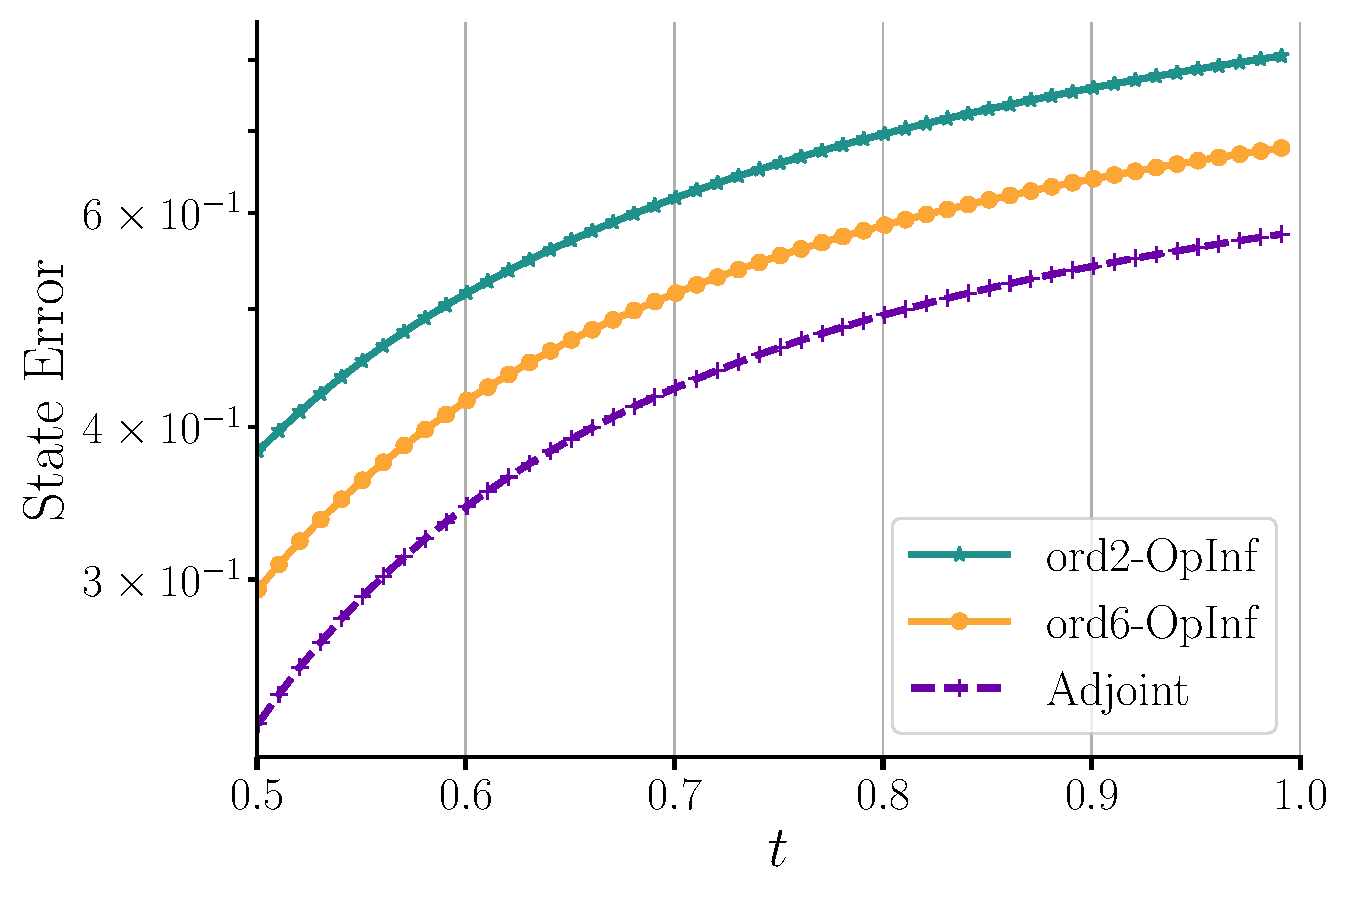
\includegraphics[width=\linewidth]{images/pred_error_vs_time_noise_10.pdf}
    \caption{10\% of noise level.}
    \label{fig:image1}
  \end{subfigure}
  \hspace{1.0cm}
  \begin{subfigure}[b]{0.3\textwidth}
    \centering
    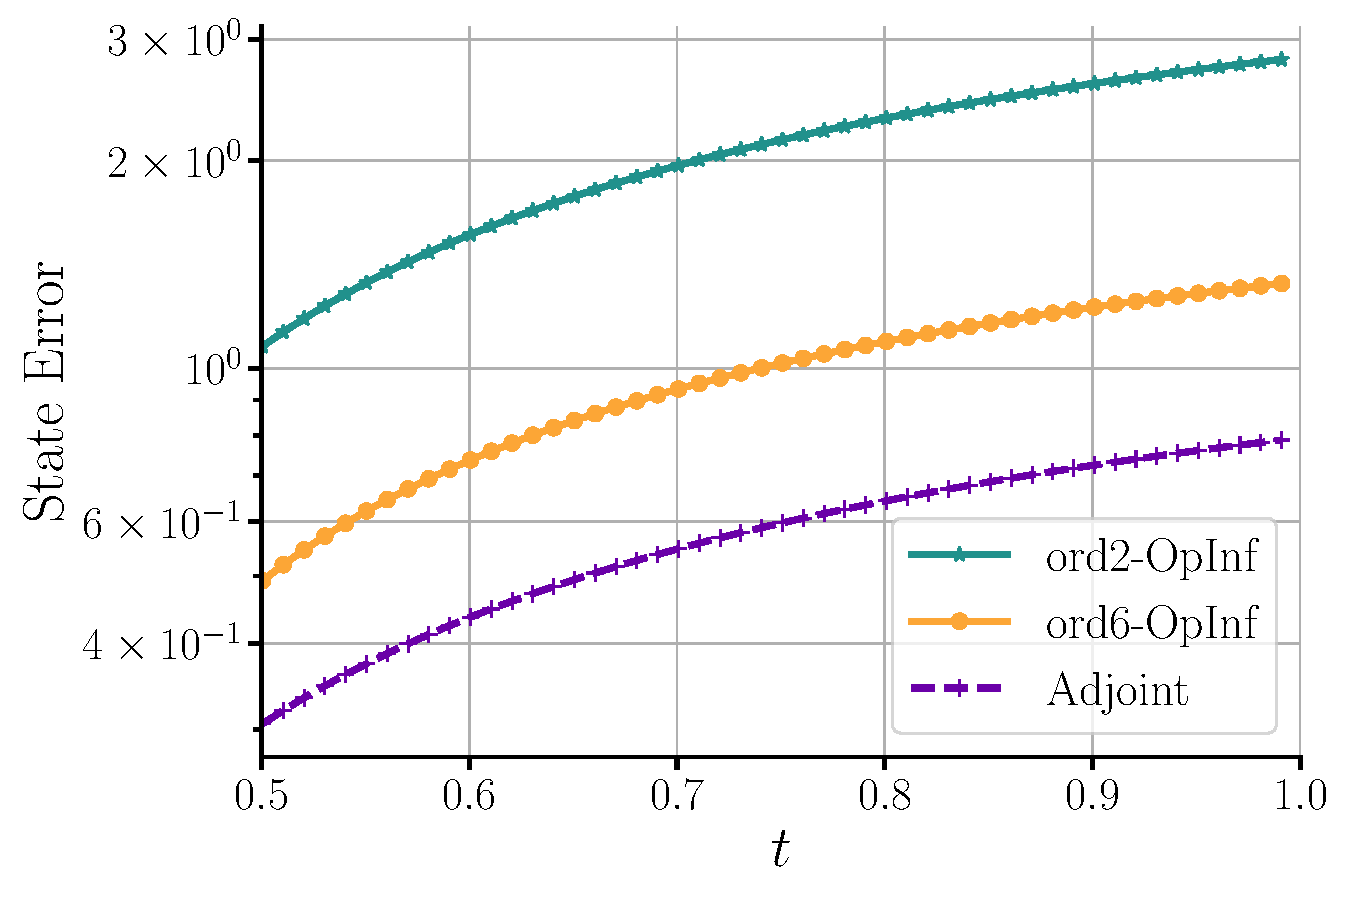
\includegraphics[width=\linewidth]{images/pred_error_vs_time_noise_20.pdf}
    \caption{20\% of noise level.}
    \label{fig:image2}
  \end{subfigure}
  
  %\vskip\baselineskip
  
  % Second row of subfigures
  \begin{subfigure}[b]{0.3\textwidth}
    \centering
    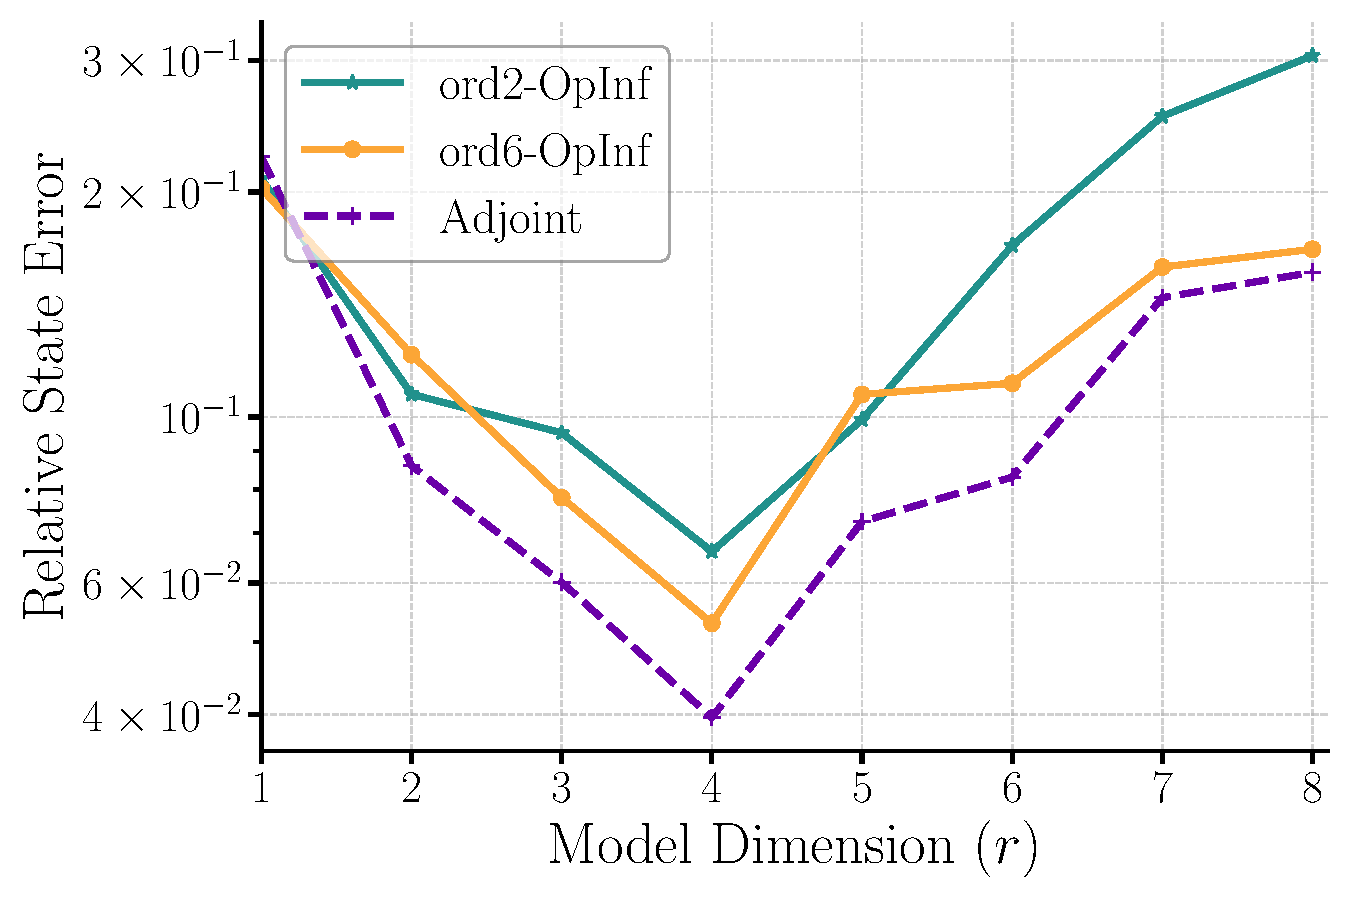
\includegraphics[width=\linewidth]{images/rel_error_vs_r_noise_10.pdf}
    \caption{10\% of noise level.}
    \label{fig:image3}
  \end{subfigure}
  \hspace{1.0cm}
  \begin{subfigure}[b]{0.3\textwidth}
    \centering
    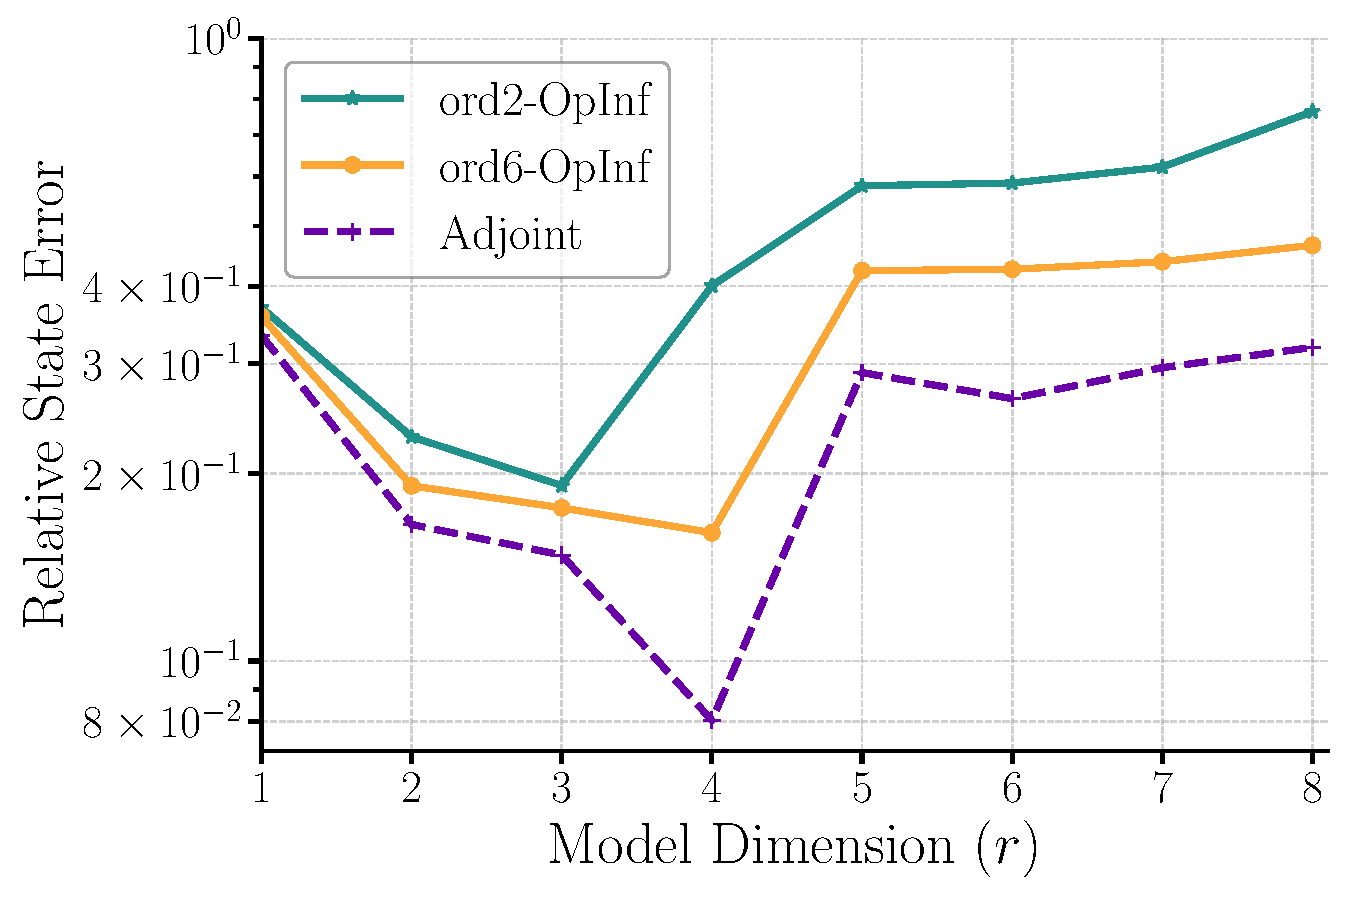
\includegraphics[width=\linewidth]{images/rel_error_vs_r_noise_20.pdf}
    \caption{20\% of noise level.}
    \label{fig:image4}
  \end{subfigure}
  
  %\caption*{caption}
  \label{fig:twobytwo1}
\end{figure}
\begin{center}
    \tiny
    (a)-(b) Prediction error vs. time; $\textbf{pred. error}=\| \hat{\mathbf{q}}_{\text{true}}(t) - \hat{\mathbf{q}}_{\text{pred}}(t) \|_2, ~t\in[0.5,1]$\\~~~~~~~(c)-(d) Relative error vs $r$; $\textbf{rel. error}=\left(\| \hat{\mathbf{q}}_{\text{true}}(t) - \hat{\mathbf{q}}_{\text{pred}}(t) \|_2\right)/\| \hat{\mathbf{q}}_{\text{true}}(t) \|_2, ~t\in[0,1]$
\end{center}

\end{frame}

\begin{frame}{FKPP Results I}
    
  \begin{columns}[T,onlytextwidth]  % top‐aligned columns, full text width
    \column{0.48\textwidth}
      \centering
      \animategraphics[loop,autoplay,width=\textwidth]{1}{images/fkpp_rom_noise_10-}{1}{2}
      \captionof*{figure}{10\% noise pertubation}
      \label{fig:left2}

    \column{0.04\textwidth}
      % just a gutter; you can adjust or even draw a rule here

    \column{0.48\textwidth}
      \centering
      \animategraphics[loop,autoplay,width=\textwidth]{1}{images/fkpp_rom_noise_20-}{1}{2}
      \captionof*{figure}{20\% noise pertubation}
      \label{fig:right2}
  \end{columns}

  \begin{itemize}
      \vspace{0.1cm} 
      \item Across varying levels of data sparsity, no significant performance gap between OpInf/Adjoint.
      \vspace{0.1cm}
      \item Under increasing noise perturbation (above figures), the Adjoint method demonstrates superior robustness in trajectory fidelity compared to OpInf
  \end{itemize}

\end{frame}

\begin{frame}{FKPP Results II}
    
\begin{figure}[h!]
  \centering
  
  % First row of subfigures
  \begin{subfigure}[b]{0.3\textwidth}
    \centering
    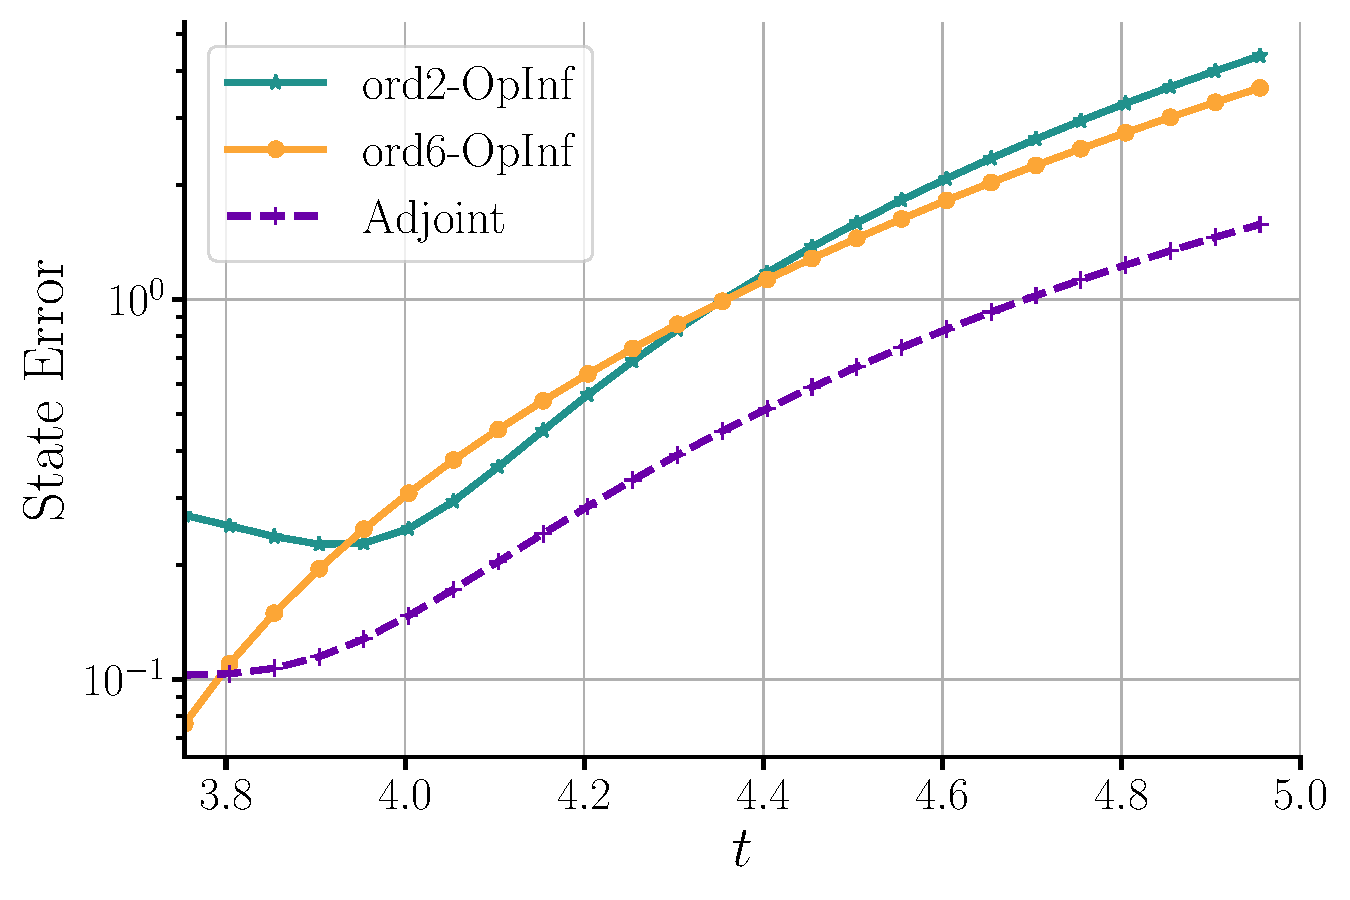
\includegraphics[width=\linewidth]{images/fkpp_pred_error_vs_time_noise_10.pdf}
    \caption{10\% of noise level.}
    \label{fig:image9}
  \end{subfigure}
  \hspace{1.0cm}
  \begin{subfigure}[b]{0.3\textwidth}
    \centering
    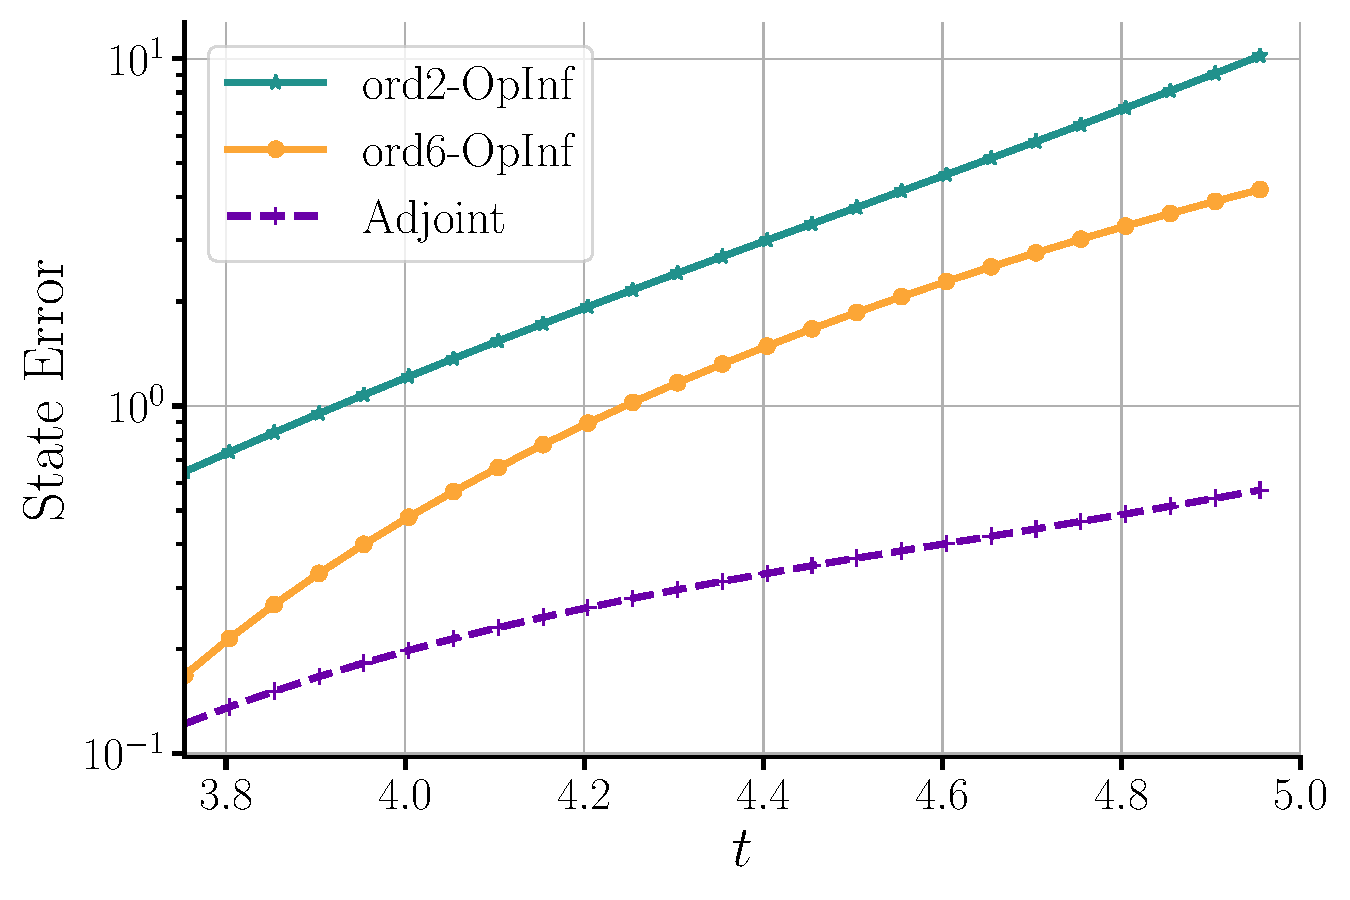
\includegraphics[width=\linewidth]{images/fkpp_pred_error_vs_time_noise_20.pdf}
    \caption{20\% of noise level.}
    \label{fig:image10}
  \end{subfigure}
  
  %\vskip\baselineskip
  
  % Second row of subfigures
  \begin{subfigure}[b]{0.3\textwidth}
    \centering
    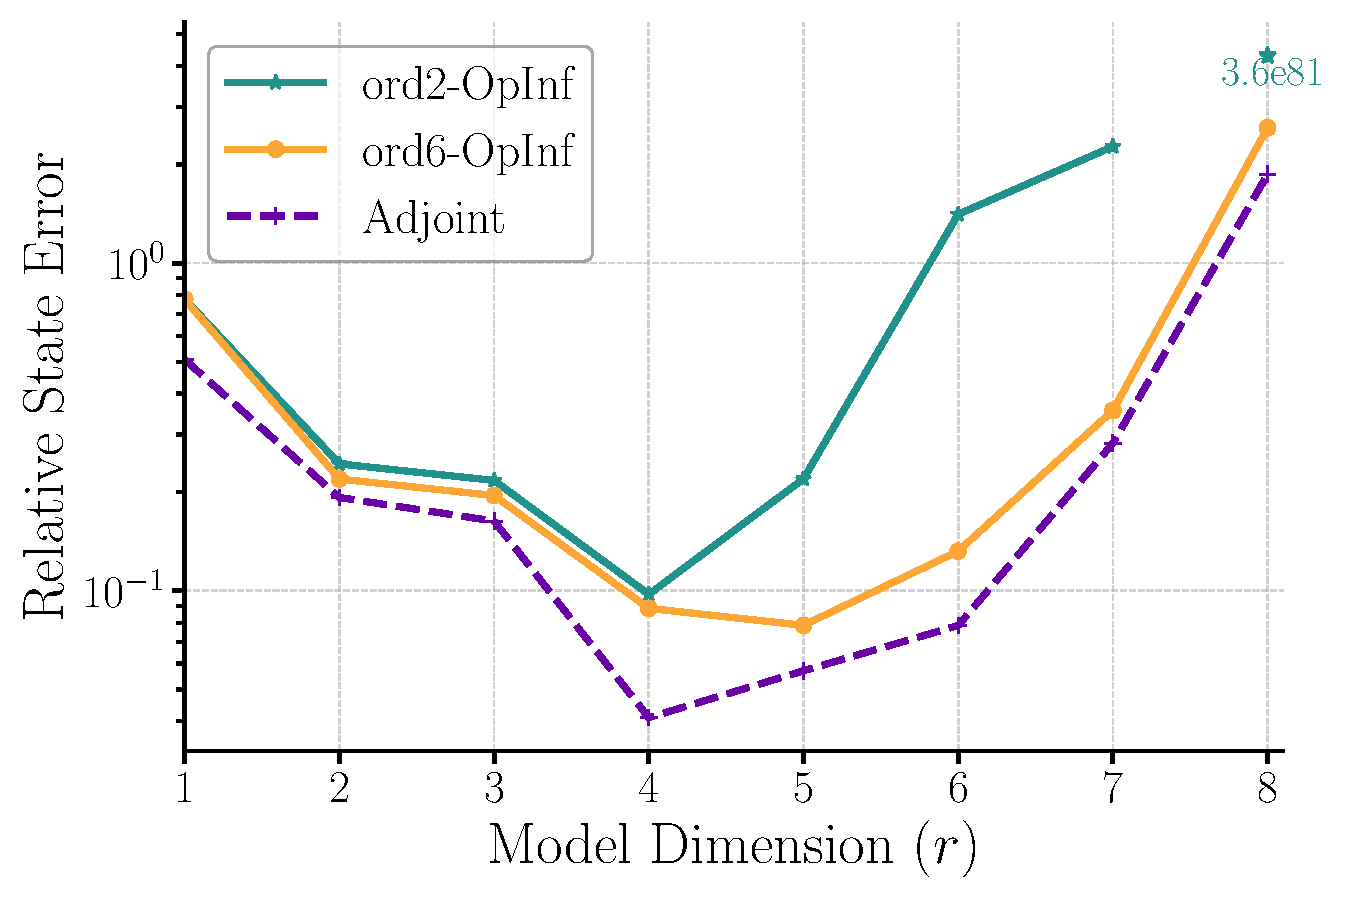
\includegraphics[width=\linewidth]{images/fkpp_rel_error_vs_r_noise_10.pdf}
    \caption{10\% of noise level.}
    \label{fig:image11}
  \end{subfigure}
  \hspace{1.0cm}
  \begin{subfigure}[b]{0.3\textwidth}
    \centering
    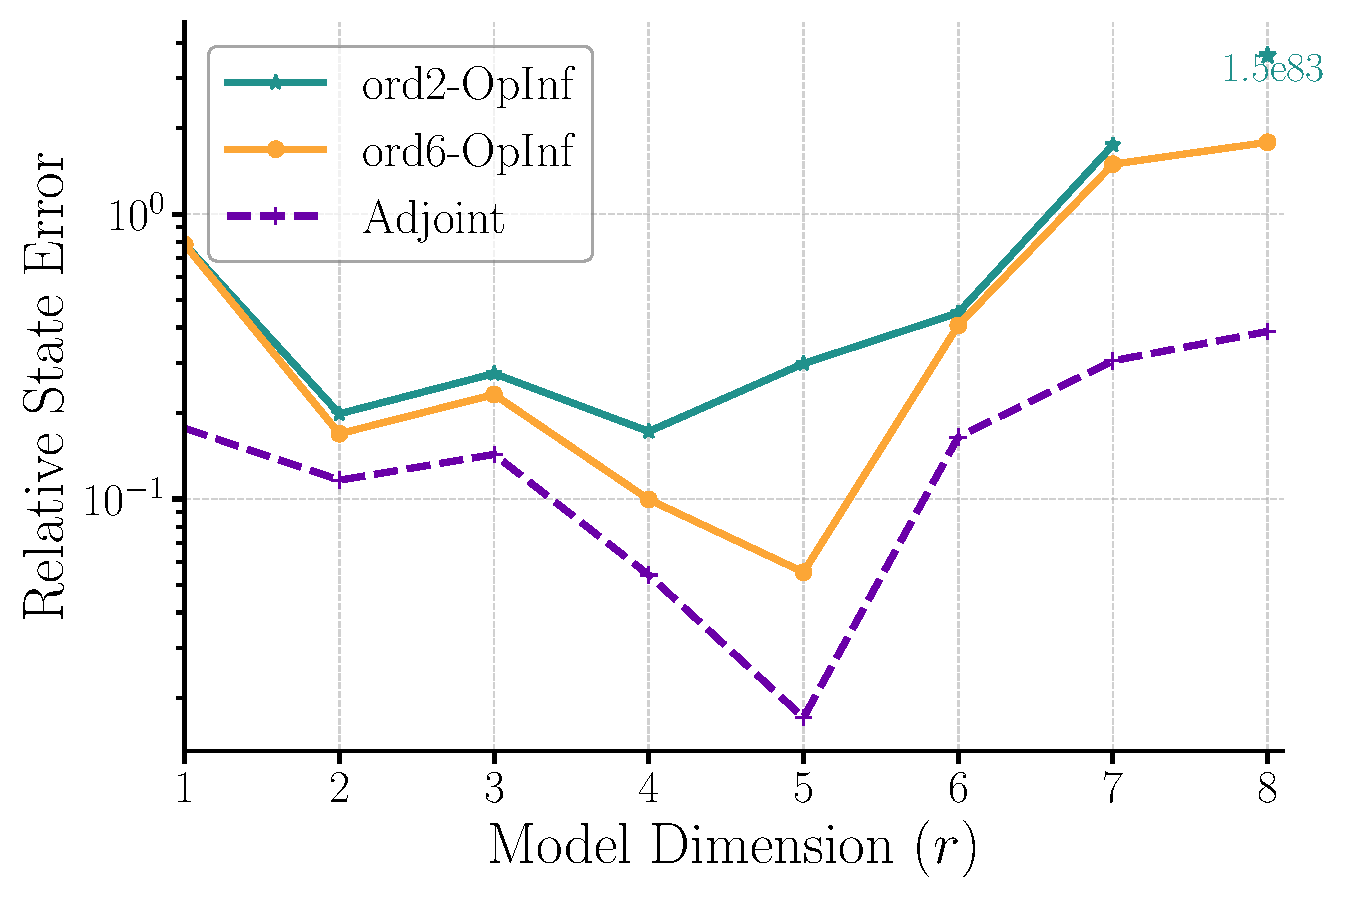
\includegraphics[width=\linewidth]{images/fkpp_rel_error_vs_r_noise_20.pdf}
    \caption{20\% of noise level.}
    \label{fig:image12}
  \end{subfigure}
  
  %\caption{Prediction error vs. time for each noise level run in the FKPP Equation experiment.}
  \label{fig:twobytwo2}
\end{figure}
\begin{center}
    \tiny
    (a)-(b) Prediction error vs. time; $\textbf{pred. error}=\| \hat{\mathbf{q}}_{\text{true}}(t) - \hat{\mathbf{q}}_{\text{pred}}(t) \|_2, ~t\in[3.75,5]$\\~~~~~~(c)-(d) Relative error vs $r$; $\textbf{rel. error}=\left(\| \hat{\mathbf{q}}_{\text{true}}(t) - \hat{\mathbf{q}}_{\text{pred}}(t) \|_2\right)/\| \hat{\mathbf{q}}_{\text{true}}(t) \|_2, ~t\in[0,5]$
\end{center}

\end{frame}